\chapter{METODOLOGI}

% Ubah konten-konten berikut sesuai dengan isi dari metodologi

\section{Metode yang digunakan}

% Contoh input gambar dengan format *.jpg
\begin{figure} [ht] \centering
  % Nama dari file gambar yang diinputkan
  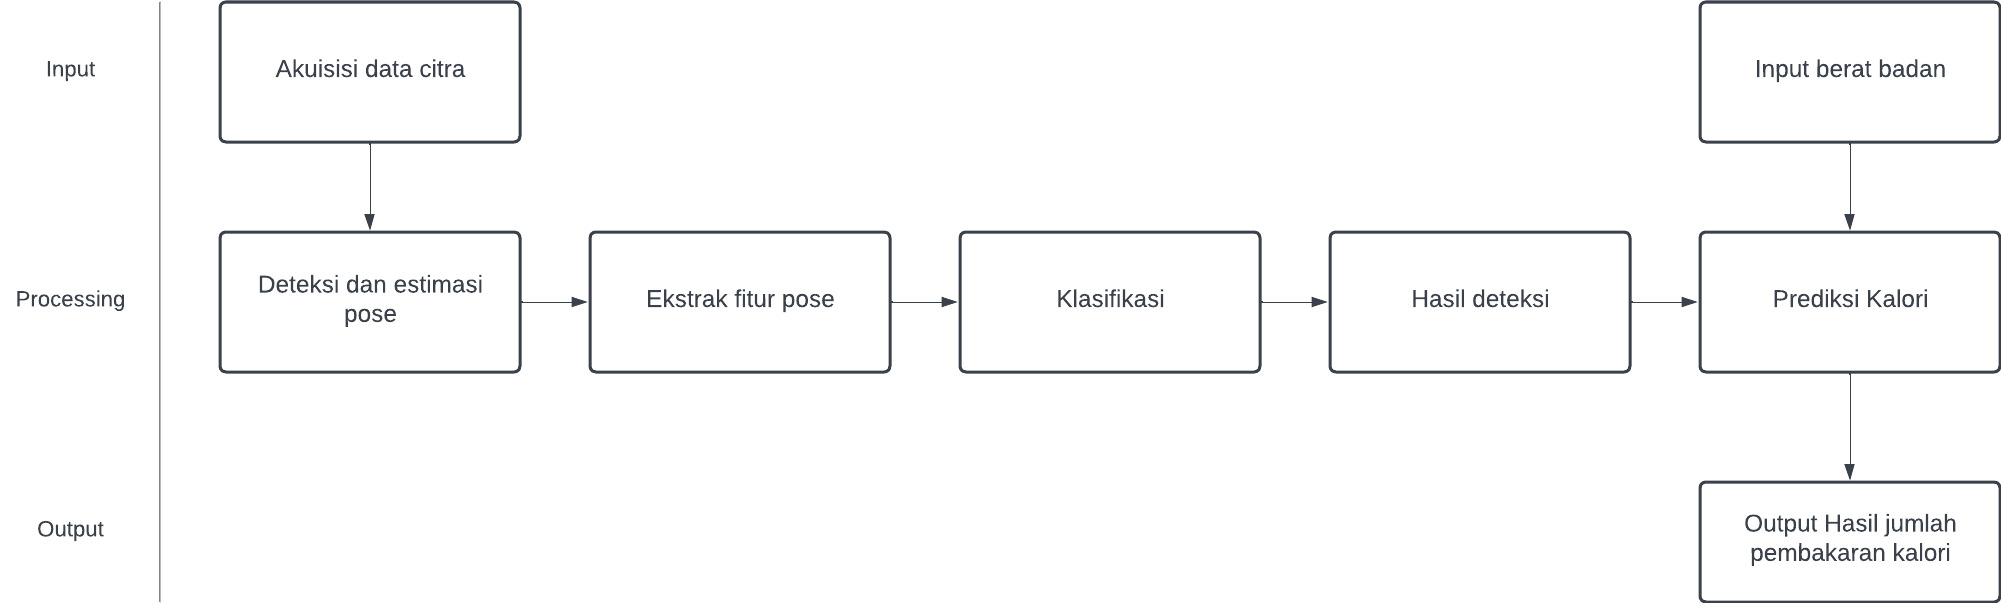
\includegraphics[scale=0.9]{gambar/blok diagram metodologi.jpeg}
  % Keterangan gambar yang diinputkan
  \caption{Blok Diagram Kerja Sistem}
  % Label referensi dari gambar yang diinputkan
  \label{fig:BlokDiagram}
\end{figure}

  \subsection{Akuisisi data citra}

  Pada tahap pertama yaitu akuisisi data citra, data diperoleh menggunakan kamera Webcam yang dimiliki oleh laptop atau kamera Webcam eksternal yang dihubungkan pada laptop ataupun komputer. Proses akuisisi data citra dilakukan dengan peraga melakukan aktivitas pada treadmill dengan ditampakkan secara jelas pada tampilan kamera Webcam. Setelah terdapat peraga dan tampak jelas pada tampilan maka data citra akan dilakukan pada tahap selanjutnya untuk dideteksi dan segmentasi pose seperti pada Gambar \ref{fig:AkuisisiData}.

  % Contoh input gambar dengan format *.jpg
  \begin{figure} [ht] \centering
    % Nama dari file gambar yang diinputkan
    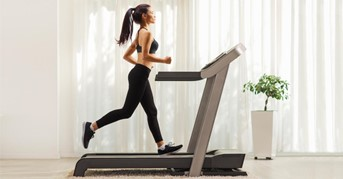
\includegraphics[scale=1.2]{gambar/akuisisi data.jpg}
    % Keterangan gambar yang diinputkan
    \caption{Posisi kamera untuk akuisisi data citra}
    % Label referensi dari gambar yang diinputkan
    \label{fig:AkuisisiData}
  \end{figure}
  
  \subsection{Deteksi dan estimasi pose}

  Deteksi dari hasil citra untuk dapat mengetahui bentuk postur tubuh manusia menggunakan Python dengan \emph{library} OpenCV yaitu MediaPipe. Metode yang digunakan pada MediaPipe menggunakan deteksi pose untuk mendeteksi postur tubuh. Segementasi dilakukan dengan cara peraga melakukan aktivitas jogging pada treadmill dengan menentukan pose melangkah seperti yang terdapat pada Gambar \ref{fig:DeteksiEstimasi}.

  % Contoh input gambar dengan format *.jpg
  \begin{figure} [ht] \centering
    % Nama dari file gambar yang diinputkan
    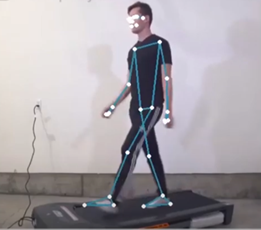
\includegraphics[scale=1.1]{gambar/deteksi estimasi.png}
    % Keterangan gambar yang diinputkan
    \caption{Deteksi dan estiasi pose dengan MediaPipe}
    % Label referensi dari gambar yang diinputkan
    \label{fig:DeteksiEstimasi}
  \end{figure}

  \subsection{Ekstrak fitur pose}

  Fitur dibuat berdasarkan segmentasi pose yang telah ditentukan dan dilakukan deteksi. Semua fitur dipersiapkan sebagai kombinasi dataset yang nantinya akan digunakan pada training. Setelah menentukan fitur yang akan diekstrak, dilakukan ekstrak fitur untuk mendapatkan setiap data yang dibutuhkan dengan setiap percobaan dari kombinasi segmentasi pose. Hasil yang didapat dari ekstrak fitur berupa data set yang nantinya akan dilakukan training untuk model yang diinginkan.

  \subsection{Klasifikasi}

  Fitur yang telah dilakukan ekstraksi maka kemudian dilakukan \emph{training} untuk memperoleh model deteksi. Model deteksi dari data set akan digunakan untuk melatih model dari sebuah algoritma pada \emph{Machine Learning}. Dalam melakukan klasifikasi menggunakan \emph{Convolutional Neural Networks} (CNN). Proses training ini bertujuan agar nantinya komputasi yang dilakukan dalam proses deteksi akan dapat diolah berdasarkan akuisisi data citra menjadi bentuk atau pola pemahaman yang diinginkan. Proses \emph{training} dilakukan dengan metode \emph{activity recognition} untuk dapat menklasifikasikan suatu aktivitas. Dengan begitu, dalam proses \emph{training} digunakan beberapa \emph{frame} dari fitur yang sudah diekstraksi untuk bisa diklasifikasikan dalam bentuk deteksi aktivitas. Klasifikasi dalam menentukan aktivitas yang digunakan pada penelitian ini adalah dapat mengetahui langkah dari seseorang yang berjalan atau berlari.

  \subsection{Hasil deteksi}

  Setelah dilakukan training dan klasifikasi, akan didapat model deteksi yang diinginkan. Bentuk hasil klasifikasi yang dibuat adalah mendeteksi pose aktivitas dengan dapat menghitung langkah dan waktu yang ditempuh. Nilai langkah dan waktu yang ditempuh akan digunakan dalam perhitungan selanjutnya.

  \begin{enumerate}[listparindent=2em]
    \item[\textbf{1.}] \textbf{Hasil deteksi langkah}
    
    Banyaknya jumlah langkah yang didapat saat hasil deteksi digunakan sebagai nilai variable pertama yang akan digunakan dalam penentuan perhitungan kalori. Langkah dideteksi dan dihitung seberapa banyak langkah yang dilakukan saat proses deteksi. Nilai banyaknya jumlah langkah akan disimpan dan akan digunakan pada saat proses perhitungan kalori setelah proses deteksi telah selesai dilakukan.

    \item[\textbf{2.}] \textbf{Hasil perhitungan waktu tempuh}
    
    Waktu tempuh saat proses deteksi merupakan nilai variabel kedua yang akan digunakan dalam penentuan perhitungan kalori. Waktu tempuh dimulai saat dideteksi pertama kali nilai langkah yang ditemukan hingga saat akhir langkah tidak ada penambahan kembali yang menandakan proses deteksi telah selesai. Nilai waktu akan dibutuhkan dalam satuan waktu menit untuk proses perhitungan kalori.

  \end{enumerate}
  
  \subsection{Prediksi kalori}

  Prediksi kalori dilakukan dengan metode regresi linear dalam menentukan dan memprediksi jumlah kalori yang terbakar berdasarkan model regresi linear yang telah ditentukan sebelumnya lalu dilakukan prediksi atas data baru yang ingin ditentukan. Dalam melakukan prediksi kalori tersebut, dilakukan beberapa tahapan untuk bisa mendapatkan dataset, model regresi, dan model prediksi untuk melakukan prediksi kalori. Adapun tahapan tersebut meliputi sebagai berikut:

  
  \begin{enumerate}[listparindent=2em]
  \item[\textbf{1.}] \textbf{Dataset jumlah kalori yang terbakar}
 
    Untuk dapat melakukan prediksi jumlah kalori yang terbakar dengan menggunakan metode prediksi maka dibutuhkan model regresi linear. Dalam pembuatan model regresi linear dibutuhkan data-data pendukung untuk dapat dilakukan model prediksi yang baik saat melakukan uji coba. Data yang dibutuhkan pada dataset sebagai variabel yang digunakan untuk model regresi maupun proses prediksi kalori adalah berat badan, waktu tempuh, jarak tempuh.

    \begin{enumerate}[label=\textbf{\alph*}., listparindent=2em]
      \item \textbf{Berat badan}
      
      Berat badan diperoleh dengan melakukan data input saat memasukkan data pada system yang digunakan. Berat badan akan berpengaruh melihat perbedaan berat badan dari seseorang yang berolahraga. Besar kecilnya nilai berat badan akan berpengaruh dikarenakan semakin besar nilai berat badan maka metabolisme tubuh untuk melakukan cepat lambatnya pembakaran kalori yang terjadi di dalam tubuh. Dengan begitu nilai berat badan akan cukup berpengaruh dalam prediksi dan perhitungan untuk menentukan jumlah kalori yang terbakar.

      \item \textbf{Waktu tempuh}
      
      Waktu tempuh diperoleh dengan menentukan dimulainya dan diakhirnya aktivitas seseorang saat berolahraga. Nilai waktu tempuh didapatkan saat melakukan proses deteksi pose pada tahap sebelumnya. Waktu tempuh juga akan mempengaruhi banyaknya kalori yang terbakar dikarenakan durasi dari seseorang melakukan kegiatan berolahraga yang semakin lama maka akan melakukan pembakaran yang semakin banyak juga.

      \item \textbf{Jarak tempuh}
      
      Jarak tempuh diperoleh dengan menetukan banyaknya langkah yang dilakukan dari seseorang yang terdeteksi dari tahap sebelumnya. Deteksi langkah yang diperoleh akan mentukan banyaknya langkah dan akan diakumulaskan untuk dikalikan dengan nilai jarak setiap langkah rata-rata. Dengan begitu akan dihasilkan nilai jarak tempuh yang dilakukan oleh seseorang yang melakukan aktivitas olahraga tersebut. Jarak tempuh digunakan untuk mengetahui bagaimana kecepatan berdasarkan jarak dibagi waktu kegiatan tersebut. Dengan mengetahui kecepatan, maka akan diketahui untuk intensitas kegiatan yang didasari oleh kecepatan berlari dari olahraga pada treadmill.
    \end{enumerate}


    \item[\textbf{2.}] \textbf{Model regresi linear}

    Regresi merupakan suatu teknik analisis untuk mengidentifikasi relasi antar dua variabel atau lebih. Regresi pada penelitian ini digunakan sebagai langkah dalam menentukan prediksi sesuai data variabel yang ditentukan. Fungsi regresi yang akan digunakan adalah dengan memodelkan dataset dan menentukan nilai prediksi dengan nilai sebenarnya. Model regresi linear dilakukan dengan cara membuat dataset terlebih dahulu yang diatur sesuai dengan variabel-variabel yang dibutuhkan pada penelitian ini. Terdapat variabel independen dan variabel dependen sebagai bentuk model dataset yang akan digunakan pada regresi linear yang digunakan. Variabel independen yang digunakan pada dataset ini adalah berat badan, waktu tempuh, dan jarak tempuh. Sedangkan untuk variabel dependen yang digunakan adalah jumlah kalori yang terbakar.

    Dalam membuat model regresi linear, perlu dilakukan training dan pencarian dataset terlebih dahulu menggunakan alat bantu treadmill yang memiliki perhitungan jumlah kalori yang terbakar. Pembuatan dataset dilakukan dengan mencoba dengan menvariasikan sebanyak-banyaknya variabel yang akan digunakan pada model regresi linear. Percobaan variabel untuk menentukan dataset dilakukan dengan variasi nilai variabel independen dengan hasil ouput dibantu dengan alat treadmill untuk nilai variabel dependen berupa jumlah kalori yang terbakar. Setelah melakukan percobaan dan pencarian dataset maka akan didapatkan dataset untuk model regresi linear.

    Model regresi linear dilakukan dengan melakukan learning terhadap dataset yang telah dibuat. Regresi itu sendiri termasuk ke dalam supervised learning yang nantinya digunakan untuk memprediksi nilai kontinu. Pola dari dataset yang sudah ditentukan akan digunakan sebagai model dengan membuat fungsi persamaan regresi linear. Proses training akan dilakukan pada Machine Learning dengan menentukan angka dari persamaan dan dibuatkan garis untuk bisa didapatkan nilai fit dari hasil data training yang telah dilakukan. Sehingga akan didapatkan model regresi linear dari dataset yang didapatkan untuk dilakukan proses prediksi kalori.

    \item[\textbf{3.}] \textbf{Proses prediksi jumlah kalori yang terbakar}

    Pada proses prediksi kalori dilakukan dengan menggunakan model regresi linear untuk dilakukan prediksi jumlah kalori. Setelah didapatkan model dengan memiliki variabel independen berupa berat badan, waktu tempuh, dan jarak tempuh, maka dalam melakukan prediksi jumlah kalori yang terbakar yang termasuk pada variabel dependen akan dapat dilakukan untuk prediksi dengan mencari nilai variabel independen untuk nantiknya akan diprediksi nilai dependen untuk nilai jumlah kalori yang terbakar. Dengan begitu saat proses deteksi dapat hanya digunakan untuk nilai yang dicari yaitu, waktu tempuh dan jarak tempuh dengan input tambahan selain deteksi berupa berat badan. Sehingga setelah melakukan proses deteksi yang menghasilkan nilai waktu tempuh, jarak tempuh, dan input berat badan akan menghasilkan prediksi jumlah kalori yang terbakar melalui model prediksi regresi linear yang sudah dibuat.

  \end{enumerate}
\subsection{Implementasi pada perangkat Singel Board Computer}

Implementasi dilakukan sebagai testing dengan akuisisi citra secara realtime menggunakan model training machine learning yang telah dibuat. Setelah proses telah berjalan dengan baik pada testing menggunakan laptop/komputer, persiapan perangkat Single Board Computer untuk dapat menampung segala kebutuhan dalam mendeteksi dan memprediksi hasil kalori yang diinginkan. Implementasi juga dapat ditambahkan dengan memberikan hasil visualisasi menggunakan user interface sebagai tampilan yang dapat divisualkan untuk mempermudah pembacaan hasil.



% \section{Bahan dan peralatan yang digunakan}

% \lipsum[13]
% \lipsum[3]

\section{Urutan pelaksanaan penelitian}

% Ubah tabel berikut sesuai dengan isi dari rencana kerja
\newcommand{\w}{}
\newcommand{\G}{\cellcolor{gray}}
\begin{table}[h!]
  \captionof{table}{Tabel timeline}
  \label{tbl:timeline}
  \begin{tabular}{|p{3.5cm}|c|c|c|c|c|c|c|c|c|c|c|c|c|c|c|c|}

    \hline
    \multirow{2}{*}{Kegiatan} & \multicolumn{16}{|c|}{Minggu} \\
    \cline{2-17} &
    1 & 2 & 3 & 4 & 5 & 6 & 7 & 8 & 9 & 10 & 11 & 12 & 13 & 14 & 15 & 16 \\
    \hline

    % Gunakan \G untuk mengisi sel dan \w untuk mengosongkan sel
    Pengambilan data &
    \G & \G & \G & \w & \w & \w & \w & \w & \w & \w & \w & \w & \w & \w & \w & \w \\
    \hline

    Pengolahan data &
    \w & \w & \w & \G & \G & \G & \w & \w & \w & \w & \w & \w & \w & \w & \w & \w \\
    \hline

    Pembuatan model prediksi &
    \w & \w & \w & \w & \w & \w & \G & \G & \G & \G & \G & \G & \w & \w & \w & \w \\
    \hline

    Uji coba dan evaluasi model prediksi &
    \w & \w & \w & \w & \w & \w & \w & \w & \w & \G & \G & \G & \G & \G & \G & \G \\
    \hline

    Penyusunan laporan &
    \G & \G & \G & \G & \G & \G & \G & \G & \G & \G & \G & \G & \G & \G & \G & \G \\
    \hline

  \end{tabular}
\end{table}


